\subsubsection{\Glspl{bearing-angle-image}}

\begin{figure}[H]
    \centering
    \tikzset{every picture/.style={line width=0.75pt}} %set default line width to 0.75pt        

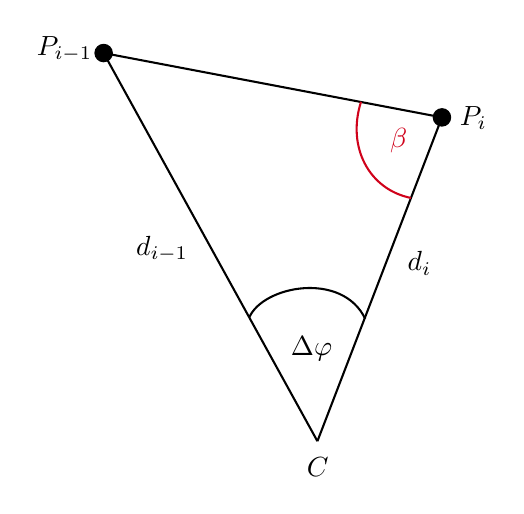
\begin{tikzpicture}[x=0.75pt,y=0.75pt,yscale=-1,xscale=1]
%uncomment if require: \path (0,227.75); %set diagram left start at 0, and has height of 227.75

%Straight Lines [id:da05017383740499093] 
\draw    (38.83,15.67) -- (141.83,202.67) ;


%Straight Lines [id:da6895513561877372] 
\draw    (201.83,46.67) -- (141.83,202.67) ;


%Curve Lines [id:da10253757735662583] 
\draw [color={rgb, 255:red, 0; green, 0; blue, 0 }  ,draw opacity=1 ]   (109,143) .. controls (115.83,127.67) and (153.83,120.67) .. (164.83,143.67) ;


%Straight Lines [id:da3851492122035306] 
\draw    (38.83,15.67) -- (201.83,46.67) ;


%Curve Lines [id:da7052636563383052] 
\draw [color={rgb, 255:red, 208; green, 2; blue, 27 }  ,draw opacity=1 ]   (162.83,39.17) .. controls (155.83,61.17) and (166.9,81.48) .. (186.9,85.48) ;


%Shape: Circle [id:dp08101382020617043] 
\draw  [fill={rgb, 255:red, 0; green, 0; blue, 0 }  ,fill opacity=1 ] (197.88,46.67) .. controls (197.88,44.49) and (199.65,42.72) .. (201.83,42.72) .. controls (204.01,42.72) and (205.78,44.49) .. (205.78,46.67) .. controls (205.78,48.85) and (204.01,50.62) .. (201.83,50.62) .. controls (199.65,50.62) and (197.88,48.85) .. (197.88,46.67) -- cycle ;
%Shape: Circle [id:dp7397482298206297] 
\draw  [fill={rgb, 255:red, 0; green, 0; blue, 0 }  ,fill opacity=1 ] (34.88,15.67) .. controls (34.88,13.49) and (36.65,11.72) .. (38.83,11.72) .. controls (41.01,11.72) and (42.78,13.49) .. (42.78,15.67) .. controls (42.78,17.85) and (41.01,19.62) .. (38.83,19.62) .. controls (36.65,19.62) and (34.88,17.85) .. (34.88,15.67) -- cycle ;


% Text Node
\draw (139,158) node [color={rgb, 255:red, 0; green, 0; blue, 0 }  ,opacity=1 ] [align=left] {$\displaystyle \Delta $$\displaystyle \varphi $};
% Text Node
\draw (181,58) node [color={rgb, 255:red, 208; green, 2; blue, 27 }  ,opacity=1 ] [align=left] {$\displaystyle \beta $};
% Text Node
\draw (191,117) node  [align=left] {$\displaystyle d_{i}$};
% Text Node
\draw (67,110) node  [align=left] {$\displaystyle d_{i-1}$};
% Text Node
\draw (217,47) node  [align=left] {$\displaystyle P_{i}$};
% Text Node
\draw (20,14) node  [align=left] {$\displaystyle P_{i-1}$};
% Text Node
\draw (142,215) node  [align=left] {$\displaystyle C$};


\end{tikzpicture}
%
    \caption[Schematic Representation of Bearing-Angles]{This figure shows the relationship of the light rays that form the \gls{bearing-angle} $\beta$.}\label{fig:bearing_angle}
\end{figure}

Scaramuzza et.al\cite{Scaramuzza2007} proposes \Glspl{bearing-angle-image} were each pixel is the angle between the current point, the optical center and the previous point.
Lin et.al\cite{Lin2017} use \Glspl{bearing-angle-image} to automatically align pointclouds using keypoints extracted with \acrshort{surf}.
Figure~\ref{fig:bearing_angle} shows the triangle that these three points form.
The neighbourhood relationship can be choosen arbitrarily resulting in four \Glspl{bearing-angle-image}, horizontal, vertical, diagonal and antidiagonal.
The second variable is the direction the angle is calculted, e.g.~for horizontal images it can be calculated from left-to-right or right-to-left.
This does not exhibit new information, because the angle of the other direction is immediatly known from the fact that the sum of the angles is $180\degree$.
Nontheless, the direction must be defined to obtain stable visual features.

The formula for the \gls{bearing-angle} $\beta$ is derived with the cosine theorem.
For the horizontal left-to-right calculation the formula is as follows.
\begin{equation}\label{eq:bearing-angle}
    \beta = \arccos%
            \frac{d_{i,j} - d_{i-1,j} \cos \Delta\varphi}%
                 {\sqrt{d_{i,j}^2 + d_{i-1,j}^2 - 2 d_{i,j} d_{i-1,j} \cos \Delta\varphi}}
\end{equation}
Note that both Scaramuzza\cite{Scaramuzza2007} and Lin\cite{Lin2017} have typos in the formulae they provided.
A full derivation for the correct equation is provided in Appendix~\ref{sec:bearing_derivation}.

The angular resolution $d\varphi$ between two pixels of the depth image depends on the camera model in use.
The pinhole models angular resolution changes between pixel pairs, equirectangular image have a constant resolution between pixels.
In general, the angle $d\varphi$ can be calculated with the spherical coordinates $P_{\mathcal{S},1}, P_{\mathcal{S},2}$ of the pixel pair $p_1, p_2$.
\begin{equation}
\begin{aligned}
    \abs{\vec{P_{\mathcal{S},1}}} &= \abs{\vec{P_{\mathcal{S},2}}} = 1 \implies P_{\mathcal{S},1} \cdot P_{\mathcal{S},2} = \cos d\varphi \\
    d\varphi &= \arccos P_{\mathcal{S},1} \cdot P_{\mathcal{S},2}
\end{aligned}
\end{equation}

The \Gls{bearing-angle} is in the range $\beta \in (0, \pi)~rad$.
Linear scaling of the angle to the color depth of the target image results in a grayscale image suitable for feature extraction.
A general scaling function for an \emph{unsigned 8bit} image and arbitrary angle range follows here.
This formulation can be used for different color depths and other potential angle calculations that result in different boundary conditions.
\begin{equation}
\begin{aligned}
\label{eq:linear_scaling}
    \beta_{min} &= 0 ~& c_{min} &= 0 \\
    \beta_{max} &= \pi ~& c_{max} &= 255 \\
    \beta_{scaled} &= \floor*{c_{min} + \beta \frac{c_{max} - c_{min}}{\beta_{max} - \beta_{min}}}
\end{aligned}
\end{equation}

\subsubsection*{Characteristics}

\begin{figure}[H]
    \begin{subfigure}[t]{0.32\textwidth}
        \includegraphics[width=\linewidth]{chapter04/img/bearing-diag-0001.png}
        \caption{This figure shows a converted \gls{bearing-angle-image} on a synthetic rendered scene.}
    \end{subfigure}
    \begin{subfigure}[t]{0.32\textwidth}
        \includegraphics[width=\linewidth]{chapter04/img/bearing-diag-0030.png}
        \caption{Rotating the camera demonstrates color changes of surfaces.}
    \end{subfigure}
    \begin{subfigure}[t]{0.32\textwidth}
        \includegraphics[width=\linewidth]{chapter04/img/bearing-diag-0210.png}
        \caption{A different camera pose result in different surface shading.}
    \end{subfigure}
    \caption[Bearing Angle Image Characteristics demonstrated]{The \gls{bearing-angle-image} is not invariant to rotation and viewpoint changes. This property limits its applicability for automatic registration of bigger discontinues changes of the camera pose. Each depth image was converted with the diagonal (top-left-to-bottom-right direction) implementation of the \gls{bearing-angle} formula.}\label{fig:bearing_characteristics}
\end{figure}
A deeper understanding of the \gls{bearing-angle-image} helps to understand advantages and disadvantages for its usage.
Figure~\ref{fig:bearing_characteristics} demonstrates the visual changes of a synthetic scene under certain camera transformations.

The most notable property is the lack of rotation invariance.
This follows directly from the definition of the \gls{bearing-angle}.
A triangle is build by a predefined pixel relationship.
Calculating the \gls{bearing-angle} from multiple directions could lead to some rotation stability, because rotations of $45\degree$ corresponds to a different direction of pixel neighbourhood.
\begin{figure}[H]
    \centering
    

\tikzset{every picture/.style={line width=0.75pt}} %set default line width to 0.75pt        

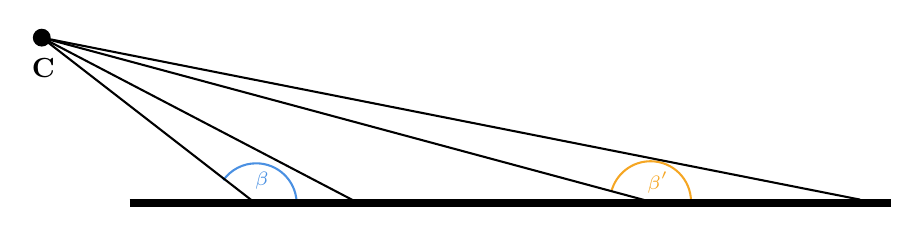
\begin{tikzpicture}[x=0.75pt,y=0.75pt,yscale=-1,xscale=1]
%uncomment if require: \path (0,111); %set diagram left start at 0, and has height of 111

%Shape: Arc [id:dp6607157958124017] 
\draw  [draw opacity=0] (294.74,88.39) .. controls (296.93,80.02) and (304.55,73.85) .. (313.6,73.85) .. controls (324.37,73.85) and (333.1,82.58) .. (333.1,93.35) -- (313.6,93.35) -- cycle ; \draw  [color={rgb, 255:red, 245; green, 166; blue, 35 }  ,draw opacity=1 ] (294.74,88.39) .. controls (296.93,80.02) and (304.55,73.85) .. (313.6,73.85) .. controls (324.37,73.85) and (333.1,82.58) .. (333.1,93.35) ;
%Shape: Arc [id:dp6461315771728425] 
\draw  [draw opacity=0] (107.76,82.98) .. controls (111.29,78.06) and (117.07,74.85) .. (123.6,74.85) .. controls (134.06,74.85) and (142.59,83.08) .. (143.08,93.42) -- (123.6,94.35) -- cycle ; \draw  [color={rgb, 255:red, 74; green, 144; blue, 226 }  ,draw opacity=1 ] (107.76,82.98) .. controls (111.29,78.06) and (117.07,74.85) .. (123.6,74.85) .. controls (134.06,74.85) and (142.59,83.08) .. (143.08,93.42) ;
%Straight Lines [id:da7912546873109455] 
\draw [line width=3]    (62.6,94) -- (429.6,94) ;
%Shape: Circle [id:dp6585955324129855] 
\draw  [draw opacity=0][fill={rgb, 255:red, 0; green, 0; blue, 0 }  ,fill opacity=1 ] (16,14.3) .. controls (16,11.93) and (17.93,10) .. (20.3,10) .. controls (22.67,10) and (24.6,11.93) .. (24.6,14.3) .. controls (24.6,16.67) and (22.67,18.6) .. (20.3,18.6) .. controls (17.93,18.6) and (16,16.67) .. (16,14.3) -- cycle ;
%Straight Lines [id:da6943190688257042] 
\draw    (20.3,14.3) -- (123.6,94.35) ;
%Straight Lines [id:da2008172675955413] 
\draw    (20.3,14.3) -- (171.6,93.35) ;
%Straight Lines [id:da41493445776640725] 
\draw    (20.3,14.3) -- (313.6,93.35) ;
%Straight Lines [id:da4646477074321278] 
\draw    (20.3,14.3) -- (414.6,92.35) ;

% Text Node
\draw (14,23) node [anchor=north west][inner sep=0.75pt]   [align=left] {$\displaystyle \mathbf{C}$};
% Text Node
\draw (121.6,77.35) node [anchor=north west][inner sep=0.75pt]  [font=\scriptsize,color={rgb, 255:red, 74; green, 144; blue, 226 }  ,opacity=1 ] [align=left] {$\displaystyle \beta $};
% Text Node
\draw (310.6,77.35) node [anchor=north west][inner sep=0.75pt]  [font=\scriptsize,color={rgb, 255:red, 245; green, 166; blue, 35 }  ,opacity=1 ] [align=left] {$\displaystyle \beta '$};


\end{tikzpicture}

%
    \caption[Two Bearing-Angles for the same ground plane]{Different shadings of plane surfaces depend on the perspective projection and the distance from the camera center $C$ to the surface.}\label{fig:bearing_angle_shading}
\end{figure}
The second apparent aspect is the change in shading for example the flat ground, but other surfaces as well.
This effect is due to the perspective transformation and the distance of a point to the camera, as Figure~\ref{fig:bearing_angle_shading} demonstrates.
Round objects, like cylinders and spheres, experience no visual change in shading.
The triangles the lightrays form with the surface are identical for such objects.
